\section{System Design and Methodology}
\label{sec:methodology}

Our proposed system employs a hierarchical Edge-Fog-Cloud architecture (illustrated in Figure~\ref{fig:system_architecture}) designed for real-time monitoring, prediction, and control of classroom environmental conditions, primarily focusing on CO\textsubscript{2} levels and occupancy.

\begin{figure}[htbp] % Use [htbp] for positioning suggestion
    \centering
    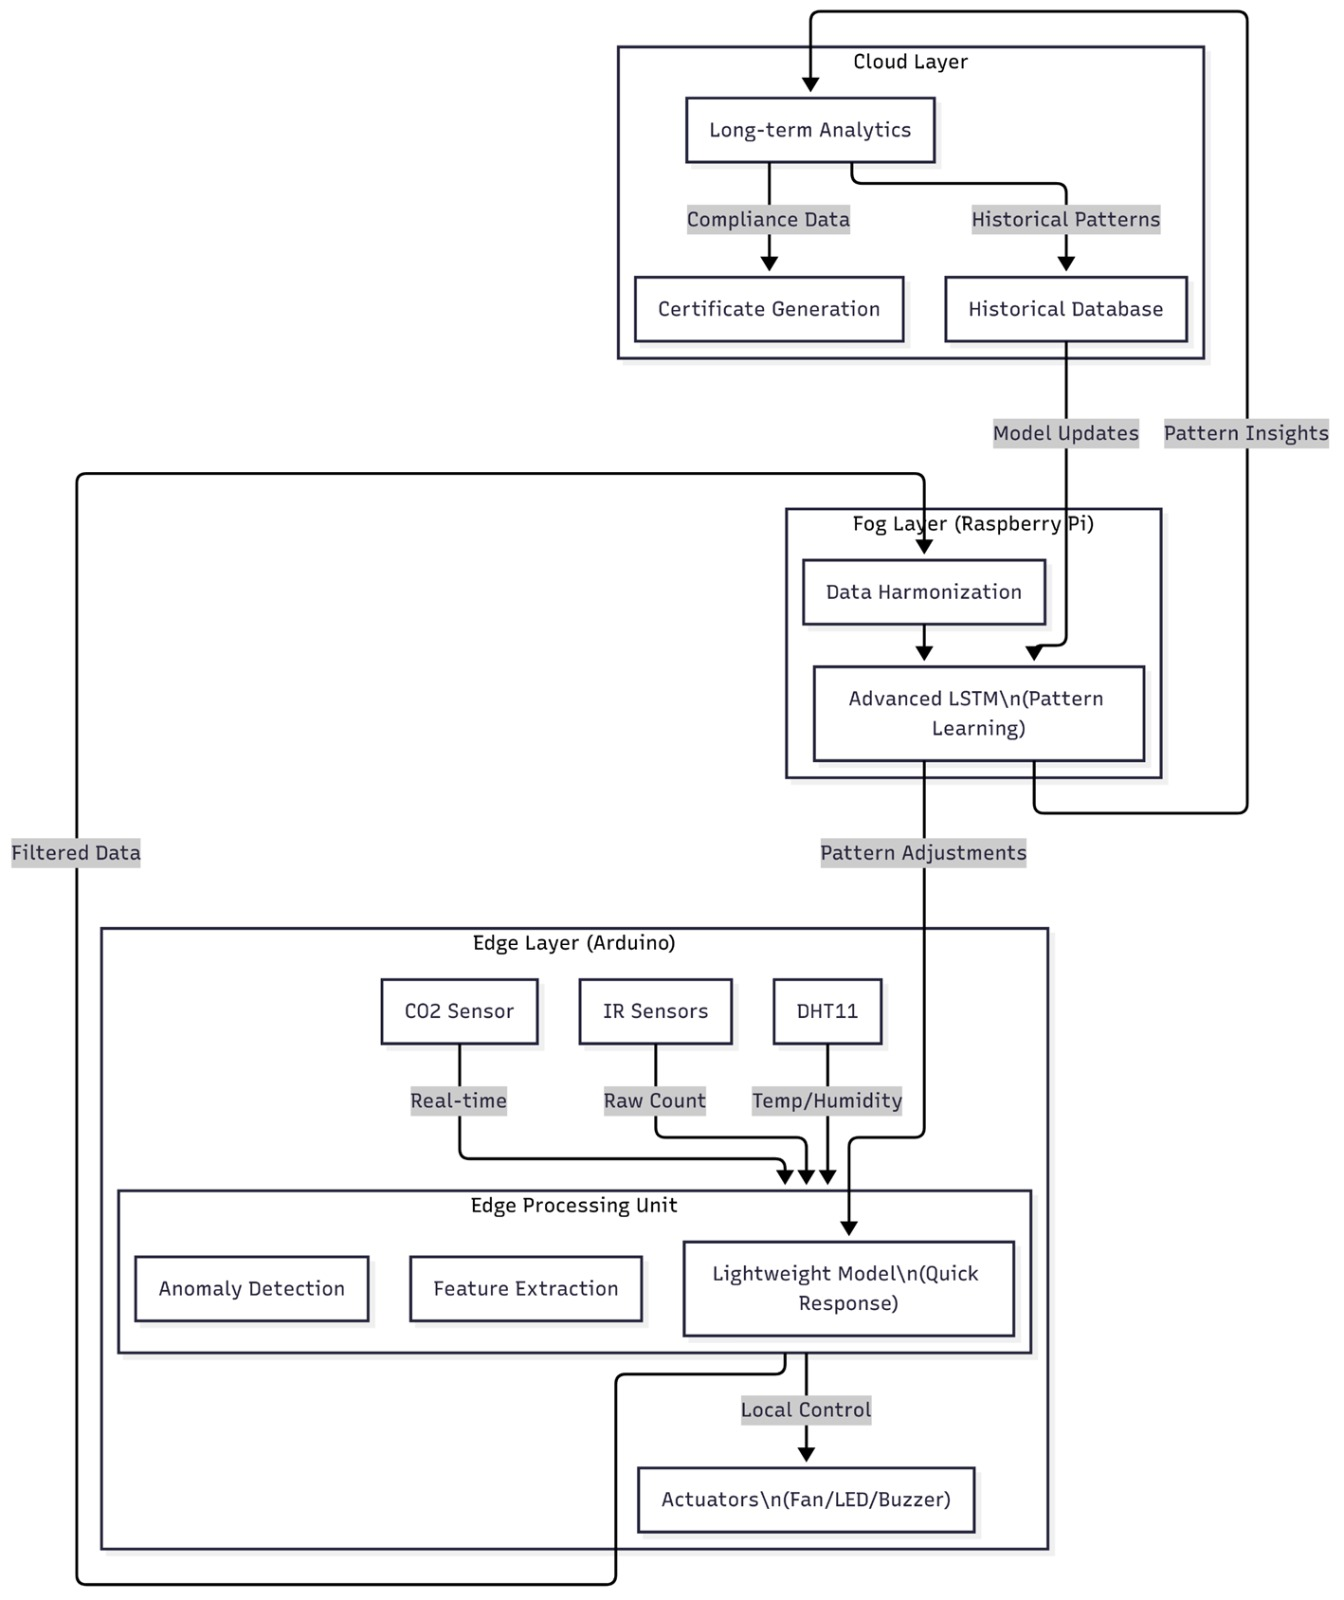
\includegraphics[width=0.9\linewidth]{figures/workflow.jpg (1).jpeg} % Use linewidth for responsiveness
    \caption{Proposed System Flow Architecture (Edge-Fog-Cloud).}
    \label{fig:system_architecture}
\end{figure}

\subsection{System Architecture}

\textbf{Edge Layer:} Consists of Arduino Uno based nodes deployed in each monitored classroom. Each node is equipped with:
\begin{itemize}
    \item An MQ135 sensor for CO\textsubscript{2} concentration measurement (400-2000 ppm range).
    \item A DHT11 sensor for temperature and humidity readings.
    \item Paired Infrared (IR) sensors at doorways for bidirectional occupancy counting.
    \item A 16x2 LCD for displaying real-time status (temperature, humidity, air quality).
    \item Actuators: 12V DC fans (controlled via relay modules), LEDs (status indicators), and buzzers (alerts).
\end{itemize}
The Arduino units perform initial data acquisition, basic filtering, local actuation (immediate response to critical thresholds), and transmit processed sensor readings to the Fog layer via serial communication (USB, 9600 baud).

\textbf{Fog Layer:} A Raspberry Pi 4 (4GB RAM) acts as the central fog controller. Its responsibilities include:
\begin{itemize}
    \item Aggregating data streams from multiple Edge nodes.
    \item Executing the pre-trained LSTM model for CO\textsubscript{2} and occupancy prediction.
    \item Implementing decision logic based on predictions and custom metrics (KPIv, Room Quality Score).
    \item Sending control commands back to Edge nodes (e.g., activate fans).
    \item Communicating with the Cloud layer for data logging and synchronization.
\end{itemize}
Python is used for programming the Fog layer, utilizing libraries like TensorFlow/TensorFlow Lite, NumPy, Pandas, and Scikit-learn.

\textbf{Cloud Layer:} ThingSpeak is utilized for cloud functionalities:
\begin{itemize}
    \item Long-term storage of historical sensor data and predictions.
    \item Data visualization through dashboards.
    \item Automated generation of environmental quality certificates based on aggregated performance data.
    \item Potential for remote monitoring and triggering model updates.
\end{itemize}

\subsection{Data Collection and Preprocessing}

Real-time data (CO\textsubscript{2}, temperature, humidity, occupancy count) is collected every few minutes (configurable, typically 3-5 mins) by the Edge nodes. Before model training (offline) and prediction (online on Fog), the data undergoes preprocessing:
\begin{itemize}
    \item Handling Missing Values: Time-based interpolation is used for offline dataset preparation.
    \item Normalization: Min-Max scaling is applied to features to ensure values are within a consistent range (e.g., 0 to 1), preventing features with larger magnitudes from dominating the learning process.
    \item Sequencing: Data is structured into sequences using a sliding window approach (e.g., using the last 10-15 timesteps) to provide temporal context for the LSTM model.
    \item Train/Validation/Test Split: For offline training, the dataset is split chronologically (e.g., 70%/20%/10%) to maintain temporal integrity.
\end{itemize}

\subsection{LSTM Predictive Model}

A Long Short-Term Memory (LSTM) network is employed for its ability to capture long-range temporal dependencies in time-series data.

\textbf{Architecture:} The model consists of:
\begin{itemize}
    \item An input layer accepting sequences of features (CO\textsubscript{2}, temperature, humidity, occupancy).
    \item Two stacked LSTM layers (64 units followed by 32 units) to learn hierarchical temporal patterns.
    \item Dropout layers between LSTM layers to mitigate overfitting.
    \item A Dense output layer producing the predicted CO\textsubscript{2} concentration for the next timestep.
\end{itemize}

\textbf{Training:} The model was trained offline using the preprocessed dataset.
\begin{itemize}
    \item Loss Function: Mean Squared Error (MSE) was used to minimize the difference between predicted and actual values.
    \begin{equation}
    \mathcal{L}_{\text{MSE}} = \frac{1}{N} \sum_{i=1}^{N} (y_i - \hat{y}_i)^2
    \label{eq:mse_methodology}
    \end{equation}
    \item Optimizer: Adam optimizer was used for efficient gradient descent.
    \item Epochs: Trained for up to 200 epochs with EarlyStopping based on validation loss to prevent overfitting.
    \item Learning Rate Scheduling: Adaptively adjusted the learning rate during training.
\end{itemize}
The trained model weights and scaler were saved (`pretrained_lstm.weights.h5`, `pretrained_scaler.joblib`) and converted to TensorFlow Lite format for efficient deployment on the Raspberry Pi (Fog layer).

\subsection{Prediction Logic and Control}

The Fog layer uses the deployed LSTM model to predict future CO\textsubscript{2} levels. Based on these predictions and current sensor readings, it calculates two key metrics:

\textbf{KPIv (Key Performance Indicator for Ventilation):} Quantifies ventilation quality based on CO\textsubscript{2} and occupancy.
\begin{equation}
KPIv = 
\begin{cases} 
2.0 & \text{if } CO_2 > 1000 \, \text{ppm} \\
\frac{CO_2 - 400}{20 \times actual\_people} & \text{if } actual\_people > 0 \\
0.5 & \text{if } est\_people > 0, actual\_people = 0 \\
0.0 & \text{otherwise}
\end{cases}
\label{eq:KPIv_methodology}
\end{equation}
where actual\_people is the count from IR sensors, and est\_people represents estimated occupancy.

\textbf{Room Quality Score:} Provides a holistic score incorporating multiple factors.
\begin{multline} 
    Score = 5 \times KPIv + 0.2 \times |Temp - 24| \\
    + 0.3 \times \frac{CO_2}{1000} + 0.1 \times Occupancy
    \label{eq:Score_methodology}
\end{multline}
This score helps compare classrooms and trigger broader actions.

Based on these metrics and predictions, the Fog layer sends commands to the Edge nodes to activate fans for ventilation, display status updates on LCDs, and trigger alerts (LEDs, buzzers) if thresholds are breached or predicted to be breached. 